\chapter{Capital Fund Management}
\label{chapter1}

\section{General presentation}
\label{chapter1_section1}


Capital Fund Management (CFM in short) is a global asset management company. It was founded in 1991 by Jean-Pierre Aguilar and Bruno Combier, two former HEC students. In 2000, CFM merged with Science and Finance, a company founded in 1994 by Jean-Philippe Bouchaud, a graduate from the French Ecole Normale Supérieure. After the demise of Jean-Pierre Aguilar in 2009 the company has been collegially managed by Jean-Philippe Bouchaud, Philippe Jordan, Marc Potters, Jacques Saulière and Laurent Laloux. 

Though CFM is based in Paris, it also has offices in New York City, London, Tokyo and Sydney. It currently employs more than 270 staff worldwide from 30 countries, most based in Paris. Its activities represent more than \$10 billions in asset management, placing it in the top 100 hedge funds in the world.

CFM takes a scientific and academic approach to finance, using quantitative and systematic techniques to develop alternative investment strategies and products for institutional investors and financial advisers. This scientific approach is combined with the latest technology to analyse large quantities of data, identify patterns, then develop and implement trading algorithms.

Academic research is at the core of CFM's activities. In particular, CFM is a pioneer of econophysics. It has innovated by applying research and academic techniques from physics to finance and economics, seeking to create consistent returns not correlated to wider market performance and applying appropriate risk parameters. CFM maintains tight links with the academic world, as demonstrated by the creation of the Capital Fund Management Chair for Econophysics and Complex Systems at Ecole Polytechnique in 2019.

CFM is primarily an investment company. Figure \ref{fig_c1_s1_1} summarizes some key figures on its investment activities.

\begin{figure}[H]
	\centering
	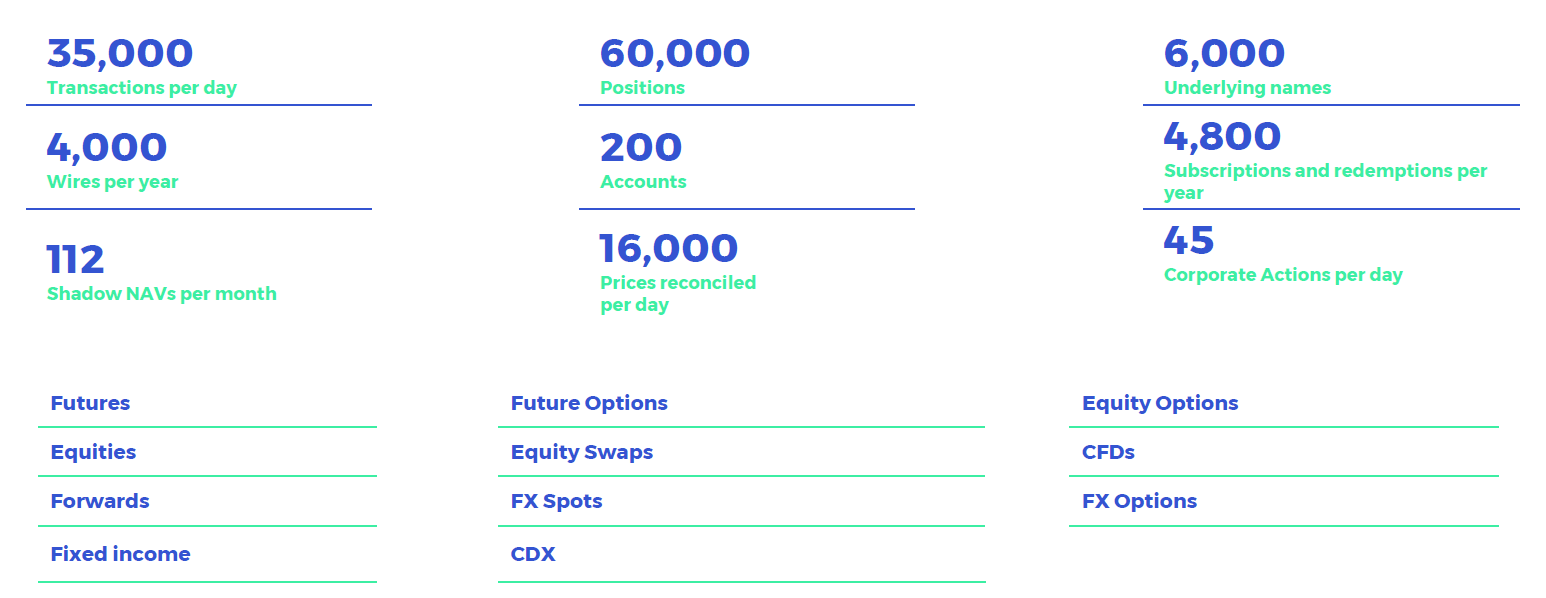
\includegraphics[scale=0.4]{images/cfm_products.png}
	\caption{Variety and volumes of products traded}
	\label{fig_c1_s1_1}
\end{figure}

In terms of investment strategies, CFM proposes two main directions. The first direction exists since 2002 and represents the range of ``hedge fund'' strategies revolving around its two main Alpha products: Stratus and Discus. These two funds are highly research-driven, and involve sophisticated proprietary models. They trade at medium frequency (daily to monthly), and involve high frequency technologies for execution. Clients of these products incur premium fees. The second direction is newer (2014) and represents the range of alternative Beta strategies. It relies on two funds: ``Long Only ESG'' (a topical investment fund with a quantitative touch), and ``Systemic Global Macro'' (a hybrid product). Strategies on these funds rely on standard models (enhanced versions), and trade more ``institutional'' products (ISD, ISE, IST, ISB...), at lower frequency. These products involve lower fees.

In short, CFM is a leading asset management company trading a wide variety and a high volume of products, using sophisticated models derived from academic research and powerful, state-of-the-art technological platforms.





